\section{Experimental Results}
\label{sec:experiment}
\begin{figure*}
\begin{center}
 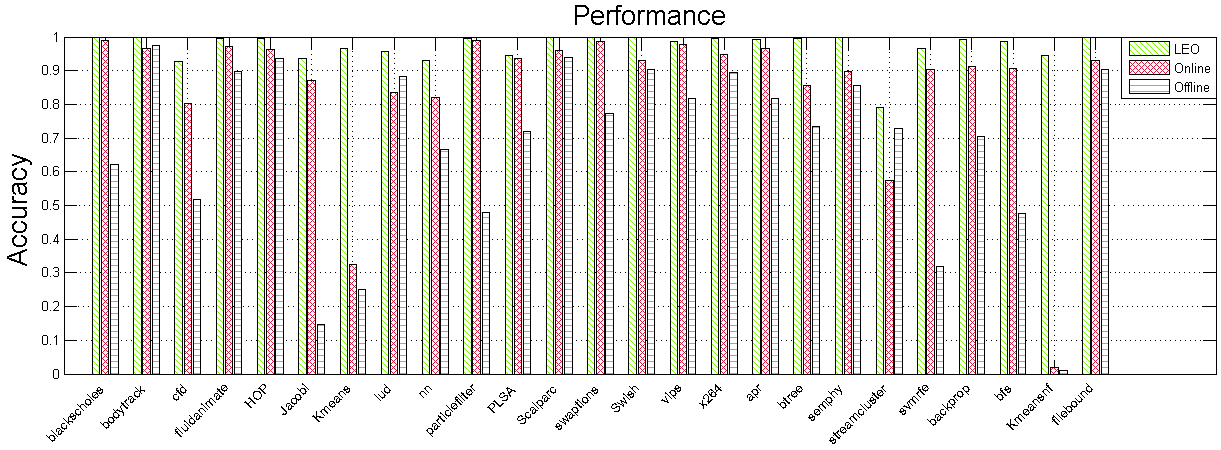
\includegraphics[width=\textwidth]{barplotPerformance.png}
 %\vspace{-7em}
 \vspace{-0.35em}
 \caption{Comparison of performance (measured as speedup) estimation
   by different techniques for various benchmarks.  \PUNT{The
     accuracies for \textit{LEO} is consistently better than
     \textit{Online} and \textit{Offline} approaches.}  On an average
   (over all benchmarks), \textit{LEO}'s accuracy is 0.97 compared to
   0.87 and 0.68 for \textit{Online} and \textit{Offline}
   respectively. The results are normalized with respect to the
   \textit{Exhaustive search} method.  }
\label{fig:barperf}
\end{center}
\end{figure*}
%\vspace{-0.35em}
\begin{figure*}
\begin{center}
 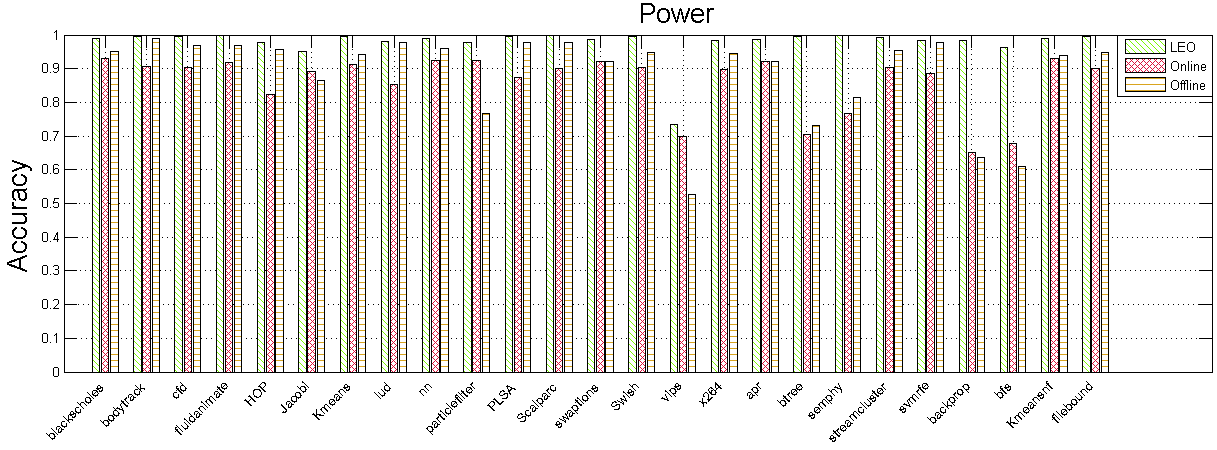
\includegraphics[width=\textwidth]{barplotPower.png}
 \vspace{-0.35em}
 \caption{Comparison of power (measured in Watts) estimation by
   different techniques for various benchmarks. \PUNT{The accuracies
     for \textit{LEO} are consistently better than the
     \textit{Offline} approach.} On an average (over all benchmarks),
   \textit{LEO}'s accuracy is 0.98 compared to 0.85 and 0.89 for
   \textit{Online} approach and \textit{Offline} approach
   respectively. Again, the results are normalized with respect to the
   \textit{Exhaustive search} method.}
\label{fig:barpower}
\end{center}
\end{figure*}
%\vspace{-0.35em}



This section evaluates \SYSTEMLEO{}'s performance and power estimates,
and its ability to use those estimates to minimize energy across a
range of performance requirements.  We begin by describing our
experimental setup and the approaches to which we compare \SYSTEMLEO{}.
We discuss \SYSTEMLEO{}'s accuracy for performance and power estimates.
We then show that \SYSTEMLEO{} provides near optimal energy savings using
these estimates.  We conclude the evaluation with a sensitivity
analysis showing how \SYSTEMLEO{} performs with respect to different
sample sizes and a measurement of \SYSTEMLEO{}'s overhead.

\subsection{Experimental Setup}
\label{sec:setup}
Our test platform is a dual-socket Linux 3.2.0 system with a
SuperMICRO X9DRL-iF motherboard and two Intel Xeon E5-2690 processors.
We use the \texttt{cpufrequtils} package to set the processor's clock
speed. These processors have eight cores, fifteen DVFS settings (from
1.2 -- 2.9 \GHz), hyper-threading, and TurboBoost.  In addition, each
chip has its own memory controller, and we use the \texttt{numactl}
library to control access to memory controllers.  In total, the system
supports 1024 user-accessible configurations, each with its own
power/performance tradeoffs\footnote{16 cores, 2 hyperthreads, 2
  memory controllers, and 16 speed settings (15 DVFS settings plus
  TurboBoost)}.  According to Intel's documentation, the thermal
design power for these processors is 135 Watts.  The system is
connected to a WattsUp meter which provides total system power
measurements at 1s intervals.  In addition, we use Intel's RAPL power
monitor to measure chip power for both sockets at finer-grain
intervals.
\begin{figure*}
\begin{center}
\begin{tabular}[t!]{ccc}\hspace*{-15pt}
	\includegraphics[width=0.3\textwidth]{performance_20_100timesmaxminYest/Kmeans.png}&
	\includegraphics[width=0.3\textwidth]{performance_20_100timesmaxminYest/Swish.png}&
	\includegraphics[width=0.3\textwidth]{performance_20_100timesmaxminYest/x264.png}\\
	{(a)} &
	{(b)} &
	{(c)}
\end{tabular}
\vspace{-0.35em}
\caption{Examples of performance estimation using \SYSTEMLEO{}.  Performance is measured as application iterations (or heartbeats) per second. (See \secref{setup}).}
\label{fig:perf}
\begin{tabular}[h]{ccc}\hspace*{-15pt}
	\includegraphics[width=0.3\textwidth]{system-power_20_100timesmaxminYest/Kmeans.png}&
	\includegraphics[width=0.3\textwidth]{system-power_20_100timesmaxminYest/Swish.png}&
	\includegraphics[width=0.3\textwidth]{system-power_20_100timesmaxminYest/x264.png}\\
	{(a)} &
	{(b)} &
	{(c)}
\end{tabular}
\vspace{-0.35em}
\caption{Examples of power estimation using \SYSTEMLEO{}. Power is
  measured as total system power. }
\label{fig:power}
\end{center}
\end{figure*}
%\vspace{-0.35em}
We use 25 benchmarks from three different suites including PARSEC
(\texttt{blackscholes}, \texttt{bodytrack}, \texttt{fluidanimate},
\texttt{swaptions}, \texttt{x264} ) \cite{parsec}, Minebench
(\texttt{ScalParC}, \texttt{apr}, \texttt{semphy}, \texttt{svmrfe},
\texttt{Kmeans}, \texttt{HOP}, \texttt{PLSA},
\texttt{non fuzzy kmeans \\* (Kmeansnf)}) \cite{minebench}, and Rodinia
(\texttt{cfd}, \texttt{nn}, \texttt{lud}, \\* \texttt{particlefilter},
\texttt{vips}, \texttt{btree}, \texttt{streamcluster},
\texttt{backprop}, \texttt{bfs}) \cite{rodinia}.  We also use a
partial differential equation solver (\texttt{jacobi}), a file
intensive benchmark (\texttt{filebound} and the \texttt{swish++}
search web-server \cite{DynamicKnobs}. These benchmarks test a range
of important multi-core applications with both compute-intensive and
i/o-intensive workloads.  All the applications run with up to 32
threads (the maximum supported in hardware on our test machine).  In
addition, all workloads are long running, taking at least 10 seconds
to complete.  This duration gives sufficient time to measure system
behavior. \PUNT{Note that various applications would work at different
  scales, hence all the data needs to be normalized so that it belongs
  to the same range.}  All applications are instrumented with the
Application Heartbeats library which provides application specific
performance feedback to \SYSTEMLEO{} \cite{Heartbeats2}. Thus
\SYSTEMLEO{} is ensured of optimizing the performance that matters to the
application.  All performance results are then estimated and measured
in terms of heartbeats/s.  In the \texttt{Kmeans} example, this metric
would represent the samples clustered per second.

To evaluate \SYSTEMLEO{} quantitatively, we measure the \emph{accuracy}
of the predicted performance and power values $\hat{\y}$ with respect
to the true data $\y$ is measured as,
\begin{equation}
\label{eq:accuracy}
\text{accuracy}(\hat{\y},\y) = \max\left(1 - \frac{\| \hat{\y}-\y \|^2_2}{\| \y - \bar{\y}\|^2_2},0\right).
\end{equation}


\subsection{Points of Comparison}
\label{sec:poc}
We evaluate \SYSTEMLEO{} in comparison to four baselines:
\begin{enumerate}
\item \textit{Race-to-idle} -- This approach allocates all resources
  to the application and once it is finished the system goes to idle.
  This strategy incurs almost no runtime overhead, but may be
  suboptimal in terms of energy, since maximum resource allocation is
  not always the best solution to the energy minimization equation
  \eqref{eq:controller}
  \cite{Carroll2013,HotPower,LeSueur11}.
\item \textit{Online} -- This strategy carries out polynomial
  multivariate regression on the observed dataset using configuration
  values (the number of cores, memory control and speed-settings) as
  predictors, and estimates the rest of the data-points based the same
  model. Then it solves the linear program given by
  \eqref{eq:controller}. This method uses only the observations and
  not the prior data.
\item \textit{Offline} -- This method takes the mean over the rest of
  the applications to estimate the power and performance of the given
  application and uses these predictions to solve for minimal energy.
  This strategy only uses prior information and we does not update
  based on runtime observations.
\item \textit{Exhaustive search} -- This brute-force approach searches
  every possible configuration to determine the true performance,
  power, and optimal energy for all applications.
\end{enumerate}

\begin{figure*}
\begin{center}
\begin{tabular}[h]{ccc}\hspace*{-15pt}
	\includegraphics[width=0.3\textwidth]{combpareto_20_100timesmaxminYest/Kmeans.png}&
	\includegraphics[width=0.3\textwidth]{combpareto_20_100timesmaxminYest/Swish.png}&
	\includegraphics[width=0.3\textwidth]{combpareto_20_100timesmaxminYest/x264.png}	\\
	{(a)} &
	{(b)} &
	{(c)}
\end{tabular}
%\vspace{-0.35em}
\caption{Pareto frontier for power and performance
  estimation using different estimation algorithms. We compare estimated Pareto-optimal frontiers to the true frontier found with exhaustive search, providing insight into how LEO solves equation \eqref{eq:controller}. When the estimated curves are below optimal plots, it represents worse performance i.e. missed deadlines, whereas the estimations above the optimal waste energy.
}
\label{fig:pareto}
\begin{tabular}[h]{ccc}\hspace*{-15pt}
	\includegraphics[width=0.3\textwidth]{LP_20_100timesmaxminYest/Kmeans.png}&
	\includegraphics[width=0.3\textwidth]{LP_20_100timesmaxminYest/Swish.png}&
	\includegraphics[width=0.3\textwidth]{LP_20_100timesmaxminYest/x264.png}\\
	{(a)} &
	{(b)} &
	{(c)}
\end{tabular}
%\vspace{-0.35em}
\caption{Energy consumption vs utilization for different
  estimation algorithms.}
\label{fig:LP}
\end{center}
\end{figure*}


\begin{figure*}
\begin{center}
 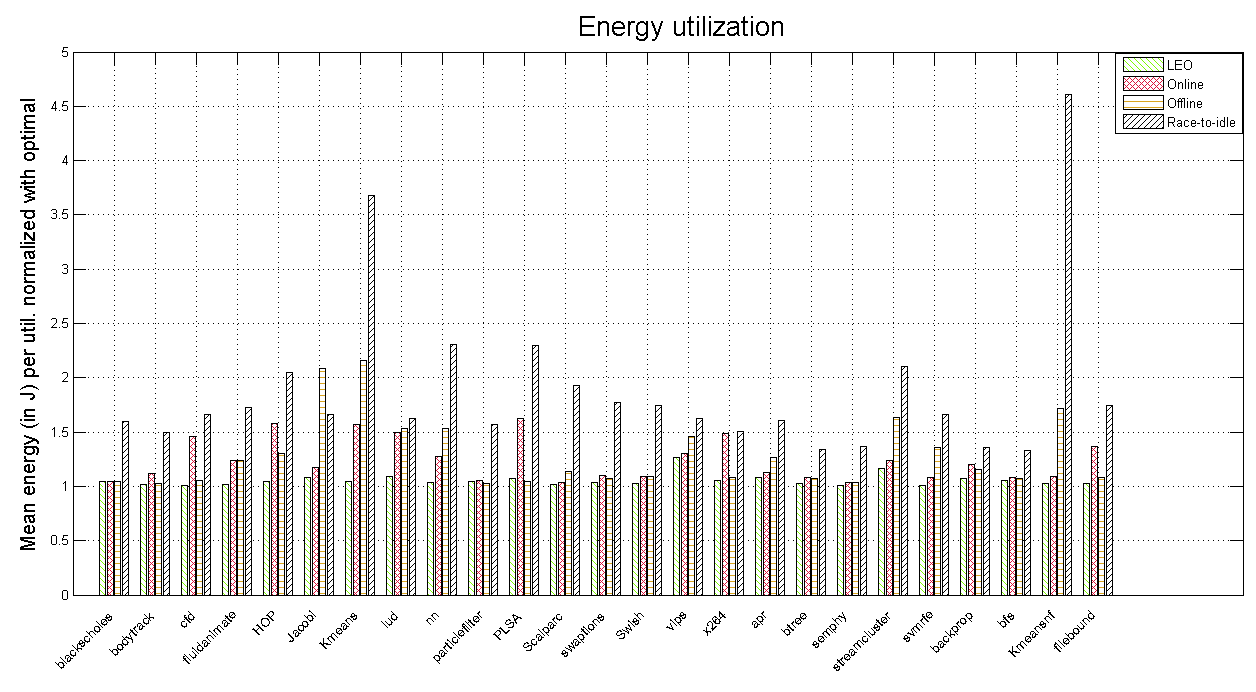
\includegraphics[width=\textwidth]{barplotEnergy.png}
 %\vspace{-0.35em}
 \caption{Comparison of average energy (normalized to
   optimal) by different estimation techniques for various benchmarks.
   \PUNT{The energy for \textit{LEO} is very close to
     \textit{Optimal}.} On an average (taken over all the benchmarks);
   \textit{LEO} consumes 6\% over optimal, as compared to the
   \textit{Online}, \textit{Offline}, and \textit{Race-to-idle}
   approaches, which respectively consume 24\%, 29\% and 90\% more
   energy than optimal. }
\label{fig:barEnergy}
\end{center}
\end{figure*}
%\vspace{-0.35em}


\subsection{Power and Performance using LEO}
\label{sec:experiment:PP}
We compare \SYSTEMLEO{}'s estimates to the \emph{online}, \emph{offline},
and exhaustive search methods described in \Secref{sec:poc}.  We deploy each of our 25 applications on our test
system and estimate performance and power.  We allow \SYSTEMLEO{} and the
online method to sample randomly select 20 configurations each. Unlike online method, which only uses these 20 samples, \SYSTEMLEO{} utilizes these 20 samples along with all the data from the other applications for the estimation purpose.  For
both \SYSTEMLEO{} and the online approach, we take the average estimates
produced over 10 separate trials to account for random variations.
The offline approach does no sampling.  The exhaustive approach
samples all 1024 configurations.

The performance and power estimation accuracies are shown in
\figref{fig:barperf} and \figref{fig:barpower}, respectively.  Each
chart shows the benchmarks on the x-axis and estimation accuracy
(computed using Equation \ref{eq:accuracy}) on the y-axis.  Unity
represents perfect accuracy.  As seen in these charts, \SYSTEMLEO{}
produces significantly higher accuracy for both performance and power.
On average -- across all benchmarks and all configurations --
\SYSTEMLEO{}'s estimations achieve $0.97$ accuracy for performance and
$0.98$ for power.  In contrast, the online approach achieves
accuracies of $0.87$ and $0.85$, while the offline approach's
accuracies are $0.68$ and $0.89$.  Even for difficult benchmarks (like
\texttt{Kmeans}), \SYSTEMLEO{} produces accurate estimations despite
sampling less than $2\%$ of the possible configuration space.

To further illustrate \SYSTEMLEO{}, we include some individual
estimations for three representative applications: \texttt{Kmeans},
\texttt{Swish}, and \texttt{x264}.  \texttt{Kmeans} is the same
application used in our example (\secref{example}), now extended to
consider all 1024 configurations of the test system.  \texttt{Swish}
is an open source search web server. \texttt{x264} is a video encoder.
All three are representative of our target applications: they are long
running and they may be launched with different performance demands.
Furthermore, all three represent some unusual trends: performance for
\texttt{Kmeans} peaks at 8 cores, for \texttt{Swish} it peaks at 16
cores, and for \texttt{x264} it is (essentially) constant after 16
cores.

Despite this behavior, \SYSTEMLEO{} produces highly accurate estimates of
performance (\figref{fig:perf}) and power (\figref{fig:power}).  Each
figure shows the configuration index on the x-axis and the predicted
performance (or power) on the y-axis.  Each chart shows both the
estimated values and the measured data points, but \SYSTEMLEO{} is so
accurate that it is hard to distinguish the two. The figures
(\figref{fig:perf} and \figref{fig:power} ) are saw-tooth in
appearance since the speed settings vary from low to high along the
\textit{Configuration index} multiple times. The saw-tooth nature of
the curves arises from two sources: (1) the extrema that naturally
arise (\eg response to cores) and (2) we have flattened a
multi-dimensional configuration space into the configuration index.
The number of memory controllers is the fastest changing component of
configuration, followed by clockspeed, followed by number of cores.
\SYSTEMLEO{} captures the peak performance configuration for all three
applications and it captures local minima and maxima.  These accurate
estimates of unusual behavior make \SYSTEMLEO{} well-suited for use in
energy minimization problems.

\subsection{Minimizing Energy}
\label{sec:experiment:LP}
%%%%%%%%%%%%%%%%%%%%%%%%% Estimation
%\vspace{-0.35em}
Our original goal, of course, is not just to estimate performance and
power, but to minimize energy for a performance (or utilization)
target.  As described in \Secref{sec:EMalg}, \SYSTEMLEO{} uses its estimates to
form the Pareto-optimal frontier of performance and power tradeoffs.
\figref{fig:pareto} shows the true convex hull and those estimated by
the \SYSTEMLEO{}, Offline and Online approaches.  Due to space
limitations, we show only the hulls for our three representative
applications: \texttt{Kmeans}, \texttt{Swish}, and \texttt{x264}.  In
these figures performance (measured as speedup) is shown on the x-axis
and system wide power consumption (in Watts) on the y-axis.  These
figures clearly show that \SYSTEMLEO{}'s more accurate estimates of power
and performance produce more accurate estimates of Pareto-optimal
tradeoffs.

To evaluate energy savings, we deploy each application with varying
performance demands.  Technically, we fix the deadline and vary the
workload $W$ from Equation \ref{eq:controller} so that $W$ $\in$
[\textit{minPerformance , maxPerformance}] for each application.  We test 100
different values for $W$ -- each representing a different utilization
demand from 1 to 100\% -- for each application.  We then use each
approach to estimate power and performance and form the estimated
convex hull and select the minimal energy configuration.

\figref{fig:LP} shows the results for our three representative
benchmarks.  Each chart shows the utilization demand on the x-axis and
the measured energy (in Joules) on the y-axis.  Each chart shows the
results for the \SYSTEMLEO{}, Online, and Offline estimators as well as
the race-to-idle approach and the true optimal energy.  As shown in
these figures, \SYSTEMLEO{} produces the lowest energy results across the
full range of different utilization targets.  \SYSTEMLEO{} is always
close to optimal and outperforms the other estimators.  Note that all
approaches do significantly better than race-to-idle. We repeat the
above experiment for all applications, then average the energy
consumption for each application across all utilization levels.  These
results are shown in \figref{fig:barEnergy}, which displays the
benchmark on the x-axis and the average energy (normalized to optimal)
on the y-axis.  On an average across all the applications, \SYSTEMLEO{}
does only 6\% worse than optimal.  In contrast, Online, Offline and
race-to-idle methods are 24\% , 29\% and 90\% worse respectively.
These results demonstrate that \SYSTEMLEO{} not only produces more
accurate estimates of performance and power, but that these estimates
produce significant -- near optimal -- energy savings.

\subsection{Sensitivity to Measured Samples}

One of the key parameters of \SYSTEMLEO{} is the number of samples it must
measure to produce an accurate estimate.  All of the above
measurements were taken with the system configured to sample 20
configurations.  In this section, we investigate the effect of the
number of configurations on the accuracy of performance and power
estimation. In \figref{fig:Sensitivity}, we show the accuracy
(averaged over all benchmarks) for performance (a) and power (b)
estimation as a function of sample size. We observe that \SYSTEMLEO{}
performs well with an even smaller sample size, whereas the Online
approach does poorly for very small sample sizes.
\begin{figure}
\begin{center}
\begin{tabular}[h]{cc}\hspace*{-15pt}
	 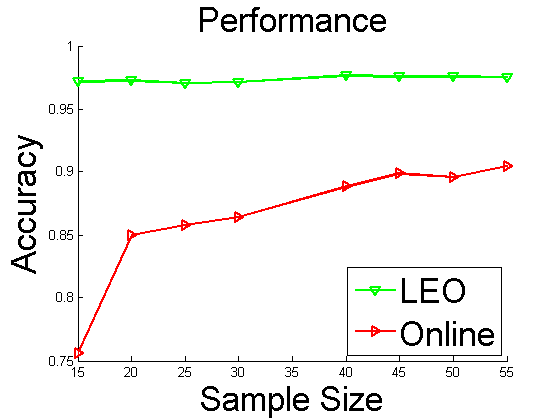
\includegraphics[width=0.5\textwidth]{AllSamplePerf.png}&
	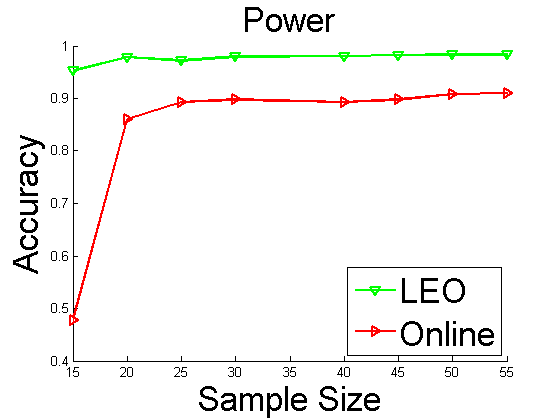
\includegraphics[width=0.5\textwidth]{AllSamplePower.png}\\
	 {(a)} &
	 {(b)}
\end{tabular}
\end{center}

\caption{Sensitivity analysis of \SYSTEMLEO{} and Online estimation. Our
  baseline method (online regression) cannot perform below 15 samples
  because the design matrix of regression model would be rank
  deficient -- effectively 0 accuracy. On the other hand, with 0
  samples, LEO behaves as the offline method and its accuracy
  increases with the sample size until it quickly reaches near optimal
  accuracy. }
\label{fig:Sensitivity}
\end{figure}
%\vspace{-0.5em}



\subsection{Reacting to Dynamic Changes}
\label{sec:controller}
%%%%%%%%%%%%%%%%%%%%%%%%%% Phases in controller



This section shows that \SYSTEMLEO{} can quickly react to changes in
application workload.  In this section we run \texttt{fluidanimate},
which renders frames, with an input that has two distinct phases.
Both phases must be completed in the same time, but the second phase
requires significantly less work.  In particular, the second phase
requires $2/3$ the resources of the first phase.  Our goal is to
demonstrate that \SYSTEMLEO{} can quickly react to phase changes and
maintain near optimal energy consumption.

\begin{figure*}
\begin{center}
\begin{tabular}[h]{cc}\hspace*{-15pt}
	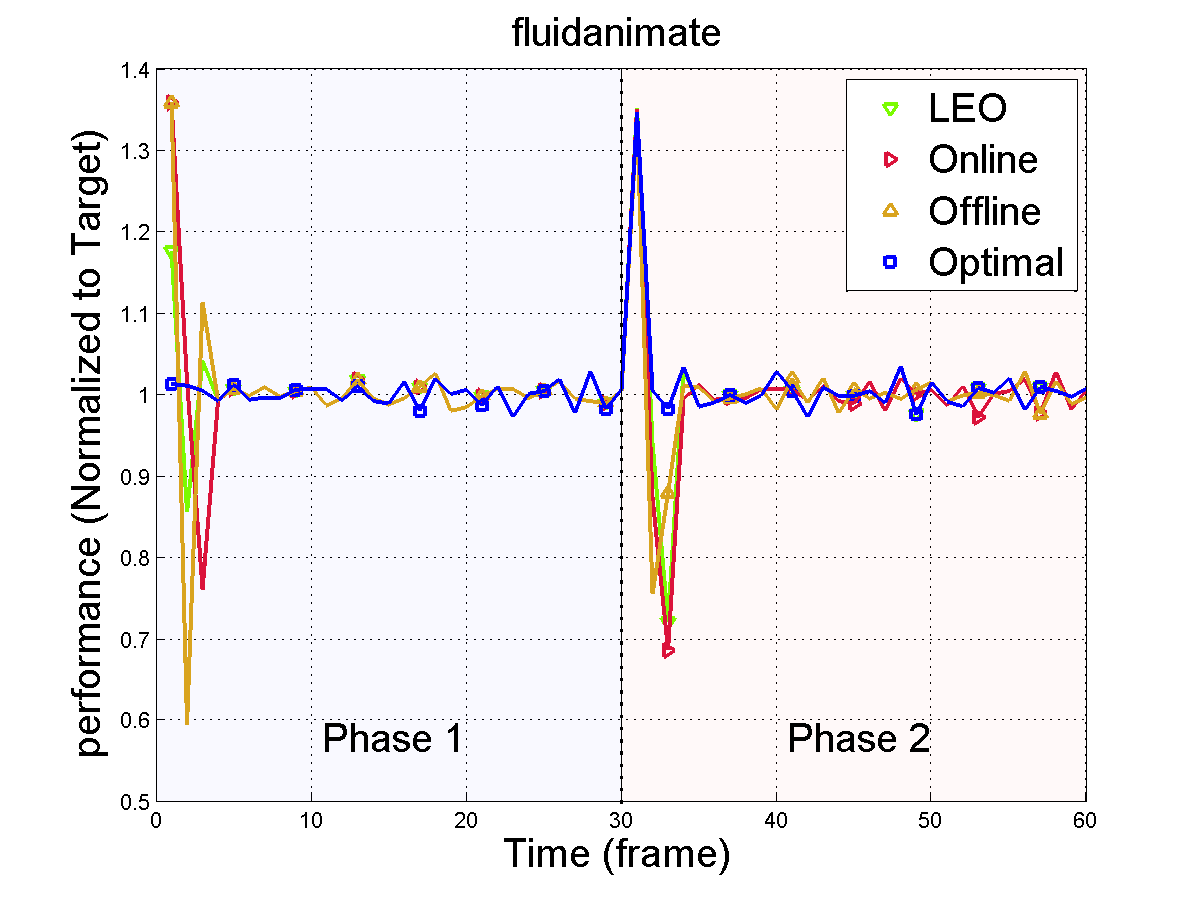
\includegraphics[width=0.5\textwidth]{Controller/fluidanimateperformance.png}&
	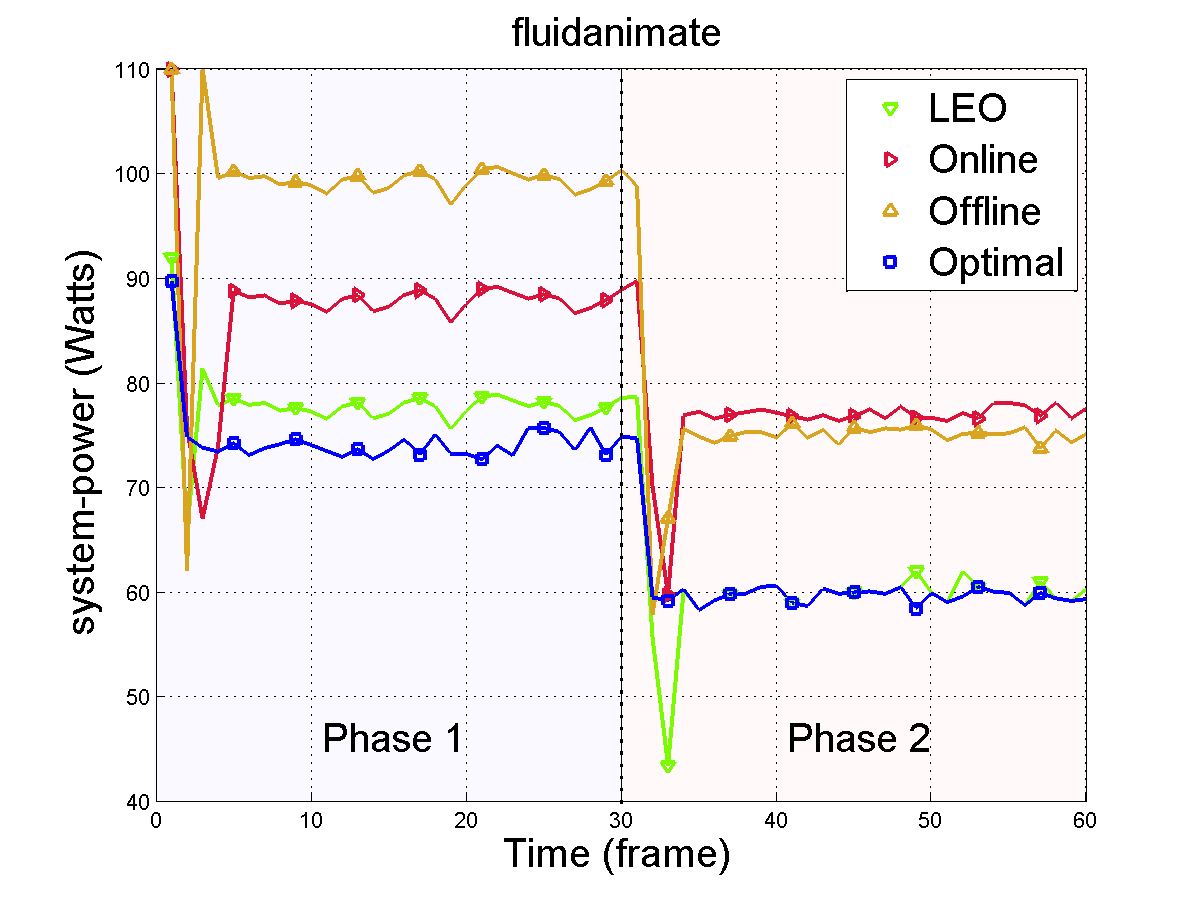
\includegraphics[width=0.5\textwidth]{Controller/fluidanimatesystem-power.png}\\
	 {(a)} &
	 {(b)}
\end{tabular}
\vspace{-0.35em}
\caption{Power and performance for \texttt{fluidanimate}
  transitioning through phases with different computational demands.}
\label{fig:phases}
\end{center}
\end{figure*}

\PUNT{
\begin{figure*}
\begin{center}
\begin{tabular}[h]{cc}\hspace*{-15pt}
	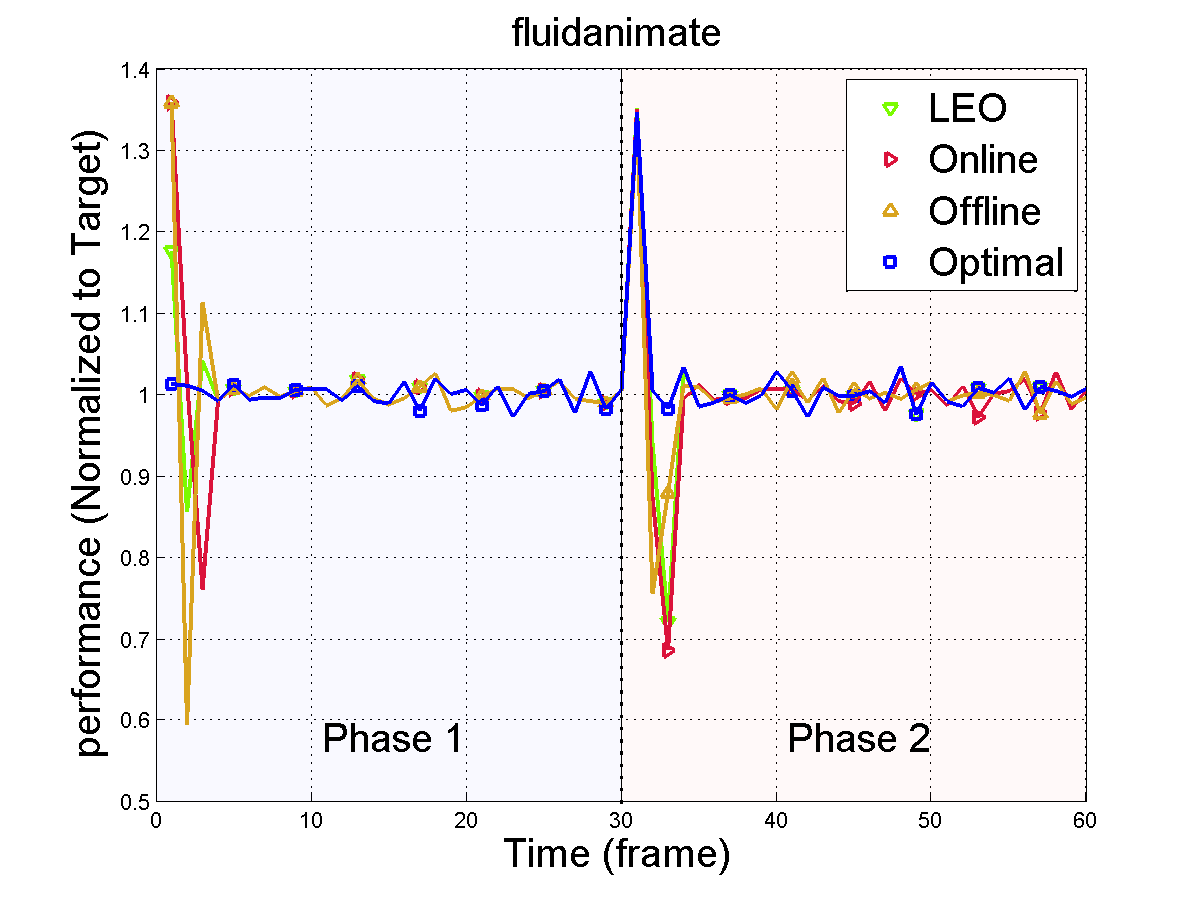
\includegraphics[width=0.45\textwidth]{Controller/fluidanimateperformance.png}&
	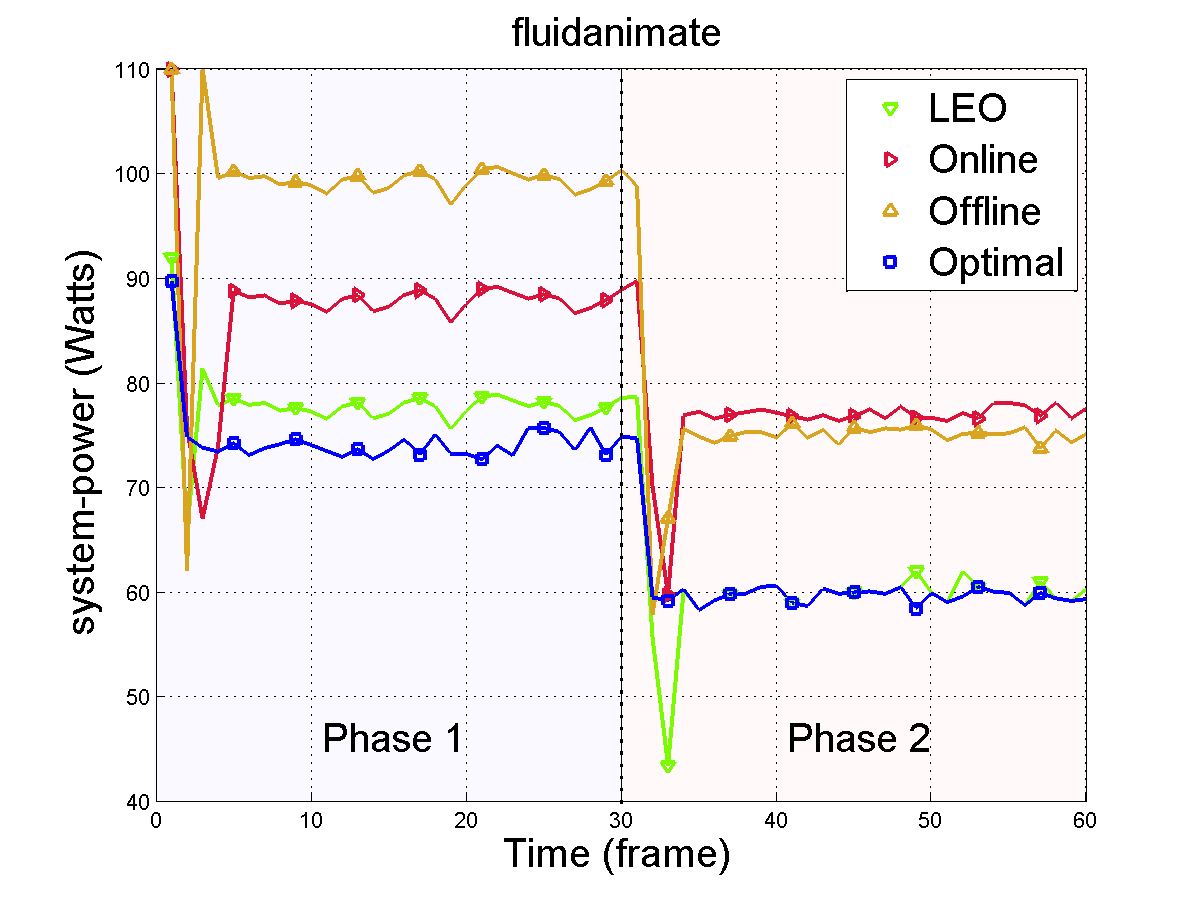
\includegraphics[width=0.45\textwidth]{Controller/fluidanimatesystem-power.png}
\end{tabular}
\vspace{-0.35em}
\caption{Power and performance for \texttt{fluidanimate}
  transitioning through phases with different computational demands.}
\label{fig:phases}
\end{center}
\end{figure*}

\begin{figure*}[t!]
    \centering
    \begin{subfigure}
        \centering
        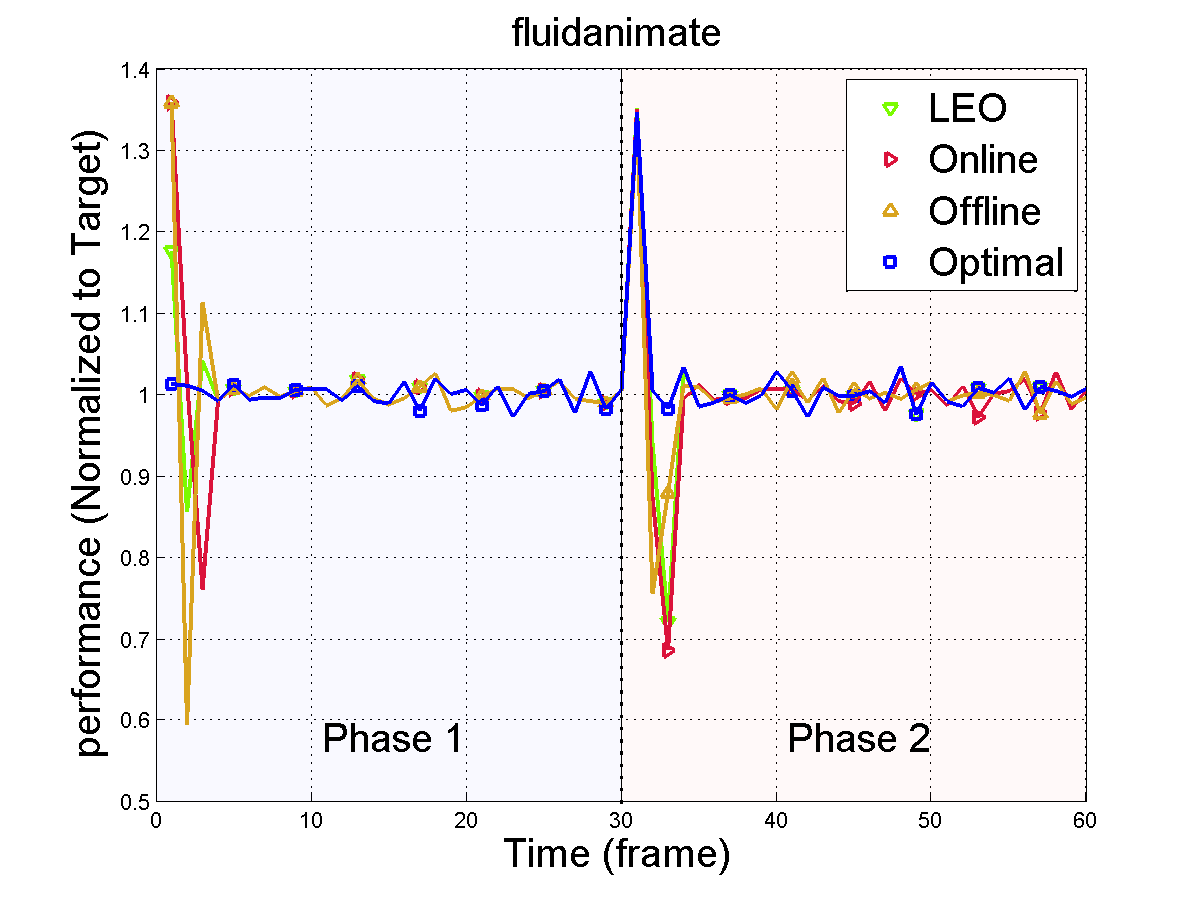
\includegraphics{Controller/fluidanimateperformance.png}
        \caption{(a)}
    \end{subfigure}%
    ~
    \begin{subfigure}
        \centering
        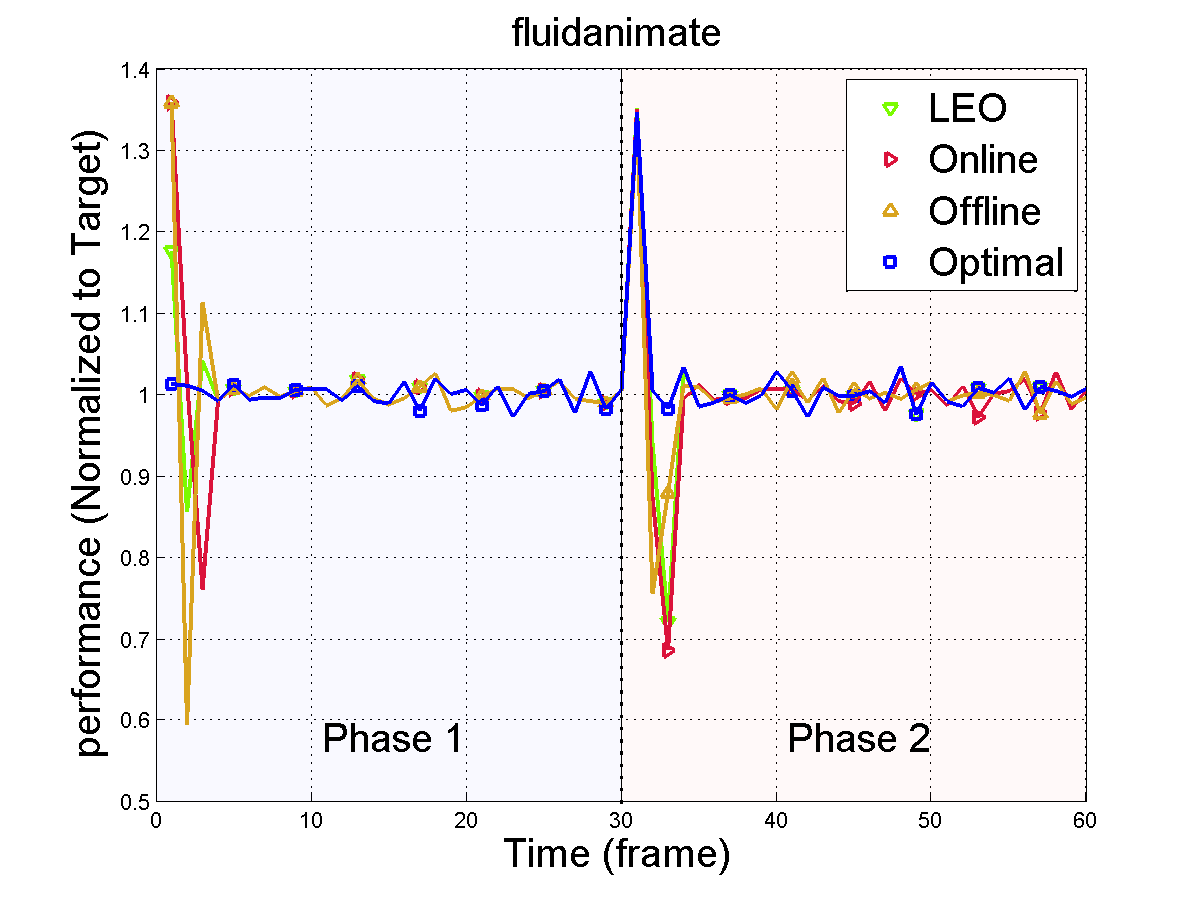
\includegraphics{Controller/fluidanimateperformance.png}
        \caption{(b)}
    \end{subfigure}
    \caption{Power and performance for \texttt{fluidanimate}
      transitioning through phases with different computational demands.}
\end{figure*}

}

\PUNT{
\begin{figure*}[t!]
    \centering
    \begin{subfigure}
        \centering
        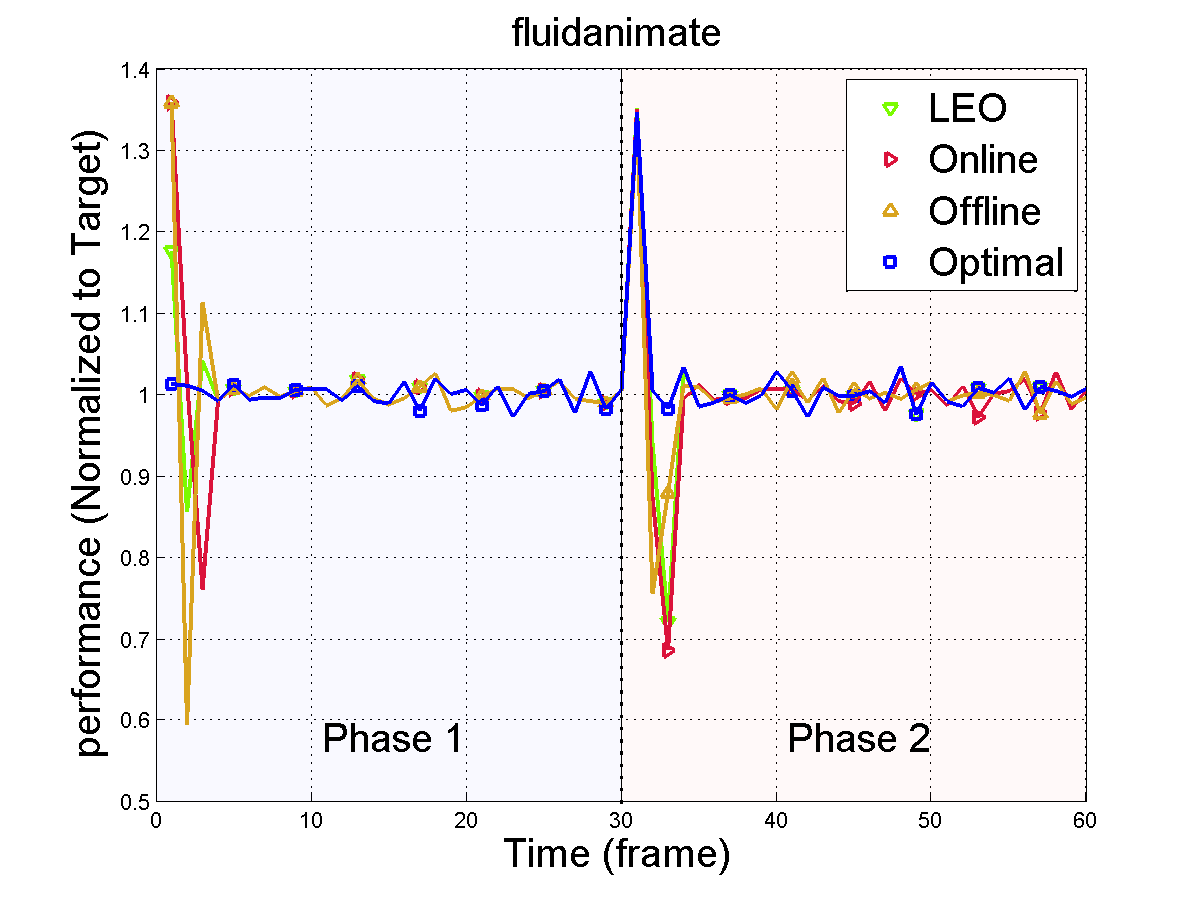
\includegraphics{Controller/fluidanimateperformance.png}
    \end{subfigure}%
    \begin{subfigure}
        \centering
        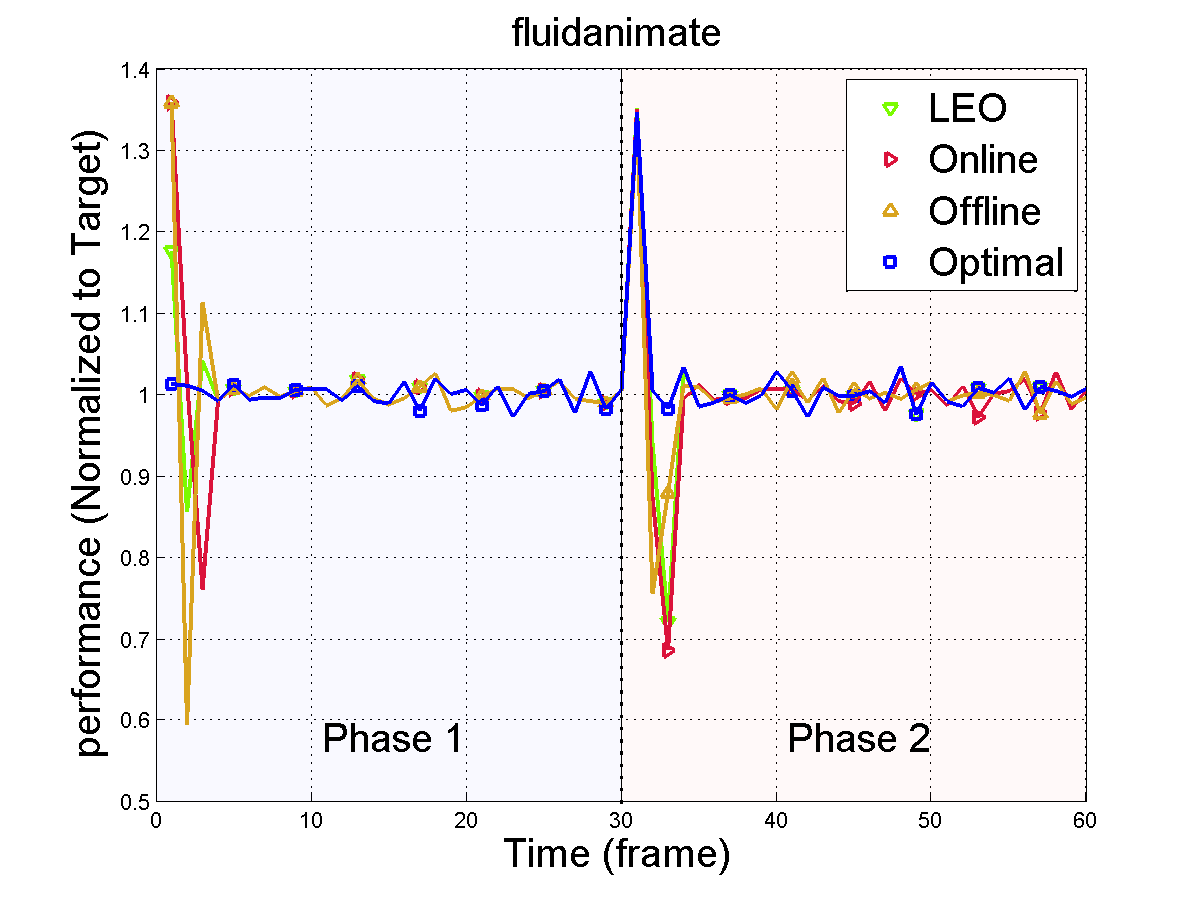
\includegraphics{Controller/fluidanimateperformance.png}
    \end{subfigure}
    \caption{Power and performance for \texttt{fluidanimate}
      transitioning through phases with different computational demands.}
\end{figure*}
}

%\vspace{-1em}

%The summarize the energy consumption in the following table.
%\vspace{-0.75em}
\begin{table}[ht]
  \caption{Relative energy consumption by various algorithms with respect to optimal.}
\centering % used for centering table
\begin{tabular}{c c c c} % centered columns (4 columns)
\hline\hline %inserts double horizontal lines
Algorithm & Phase\#1 & Phase\#2 & Overall \\ [0.5ex] % inserts table %heading
\hline % inserts single horizontal line
\text{LEO} & 1.045 & 1.005 & 1.028 \\ % inserting body of the table
\text{Offline} & 1.169 & 1.275 & 1.216 \\
\text{Online} & 1.325 & 1.248 & 1.291 \\
\hline %inserts single line
\end{tabular}
\label{tbl:nonlin} % is used to refer this table in the text
\end{table}


The results of this experiment are shown in \figref{fig:phases}.  Each
chart shows time (measured in frames) on the x-axis.
\figref[a]{fig:phases} shows performance normalized to real-time on the
x-axis, while \figref[b]{fig:phases} shows power in Watts (subtracting out
idle power) on the y-axis.  The dashed vertical line shows where the
phase change occurs.  Each chart shows the behavior for \SYSTEMLEO{},
Offline, Online, and optimal approaches.

All approaches are able to meet the performance goal in both phases.
This fact is not surprising as all use gradient ascent to increase
performance until the demand is met.  The real difference comes when
looking at power consumption, however.  Here we see that \SYSTEMLEO{}
again produces near optimal power consumption despite the presence of
phases.  Furthermore, this power consumption results in near optimal
energy consumption as well, as shown in \tblref{nonlin}.  These
results indicate that \SYSTEMLEO{} produces accurate results even in
dynamically changing environments.



\subsection{Overhead}
\label{sec:experiment:overhead}
\PUNT{ \SYSTEMLEO{}'s runtime overhead is tricky to quantify.  } The
runtime takes several measurements, incurring minuscule sampling
overhead.  After collecting these samples, it incurs a one-time cost
of executing \SYSTEMLEO{}.  After executing this algorithm, the models
are sufficient for making predictions and \SYSTEMLEO{} does not need to
be executed again for the life of the application under control.  This
is the reason we believe \SYSTEMLEO{} is best suited for long running
applications which may operate at a range of different utilizations.
The one-time estimation process is sufficient to provide accurate
estimates for the full range of utilizations (see
\Secref{sec:experiment:LP}).

Therefore, we measure overhead in two ways.  First, we measure the
average time required to execute \SYSTEMLEO{} on our system.  The average
execution time is 0.8 seconds across each benchmarks for each power
and performance.  \PUNT{ This power consumption is low because we have
  not parallelized the runtime to take full advantage of the available
  cores on our system.\TODO{Not sure here} } Second, we measure the
average total system energy consumption while executing the runtime,
obtaining an energy overhead of 178.5 Joules. These overheads are not
trivial, and they indicate (as stated in the introduction) that
\SYSTEMLEO{} is not appropriate for all deployments.  For applications
that run in the 10s of seconds to minutes or more, however,
\SYSTEMLEO{}'s overheads are easily amortized by the large energy savings
it enables.  For comparison, the exhaustive search approach takes more
than 5 days to produce the estimates for \texttt{semphy}.  For the
fastest application in our suite, \texttt{HOP}, exhaustive search
takes at least 3 hours.
